\documentclass[10pt,a4paper]{article}
\usepackage[utf8]{inputenc}
\usepackage[T1]{fontenc}
\usepackage{amsmath,amssymb,amsthm}
\usepackage{amsfonts}
\usepackage{amssymb}
\usepackage{graphicx}
\usepackage{cancel}
\theoremstyle{definition}
\newtheorem{defi}{Definition}[section]
\newtheorem*{notat}{Notation}
\newtheorem{exi}{Example}[section]
\newtheorem{teo}{Theorem}[section]
\newtheorem*{rem}{Remark}
\newcommand{\indep}{\perp \!\!\! \perp}
\newcommand{\questeq}{\stackrel{?}{=}}
\usepackage{xcolor}
\usepackage{dsfont}
\newcommand{\ind}{\mathds{1}}
\usepackage{tikz}

\usepackage{graphicx}
\graphicspath{ {./images/} } % Path relative to the main .tex file 
\usepackage{float}
\usepackage{caption}

\newcommand{\fg}[3][\relax]{%
  \begin{figure}[H]%[htp]%
    \centering
    \captionsetup{width=0.7\textwidth}
      \includegraphics[width = #2\textwidth]{#3}%
      \ifx\relax#1\else\caption{#1}\fi
      \label{#3}
  \end{figure}%
  %\FloatBarrier%
}

\begin{document}
	%\maketitle	Martingales
	\section{Conditional Expectation}
%	\begin{Prop}
		$(\Omega,\mathcal{F},\mathbb{P})$  probability space. \\
		$\mathcal{G}\subseteq\mathcal{F}$           $ \mathcal{G}$ sub-$\sigma$-algebra of  $\mathcal{F} $ .\\
		$ X:\Omega\to\mathbb{R} $ random variable with $ \mathbb{E}[|X|]<+\infty .$
		\begin{defi}
			We call conditional expectatiom of $X$ w.r.t. $\mathcal{G}$ any $\mathcal{G}$-measurable random variable $ V $ s.t.:
			\begin{equation}
				\int_{G}X\mathrm{d}\mathbb{P} = \int_{G}V\mathrm{d}\mathbb{P}  \qquad    \forall G \in \mathcal{G}
			\end{equation}
		\end{defi}
		\begin{notat}
			$V=\mathbb{E}[X|\mathcal{G}]$.
		\end{notat}
	\begin{exi}
		$X_1...X_n$  $ B(1,p) $ independent   $ S_n= X_1+...+X_n$ \\
		$\mathcal{G}=\sigma(S_n)$ $\sigma$-algebra generated by the events $ \{S_n=k\}$   $ k=0...n$ 
		\begin{equation*}
			\forall i\in {1...n}  \quad  \mathbb{E}[X_i|\sigma(S_n)]=\frac{S_n}{n}  \left(\text{another notation } \mathbb{E}[X_i|S_n=k]=\frac{k}{n}\right) 
		\end{equation*}
	\end{exi}
\begin{proof}
Any set in $\mathcal{G}$ is union of $ {S_n=k} $ for some $ k $'s. Therefore it suffices to show that:
\begin{equation*}
	\int_{{S_n=k}}X_i\mathrm{d}\mathbb{P} = \int_{{S_n=k}}\frac{S_n}{n}\mathrm{d}\mathbb{P}  \qquad    \forall k=0...n
\end{equation*}
$ X_i  $ has values in $ \{0,1\} $ so
\begin{equation*}
	\int_{\{S_n=k\}}\ind_{\{X_i=1\}}\mathrm{d}\mathbb{P} = \frac{k}{n}\cdot\mathbb{P}\{S_n=k\}   \qquad   \forall k=0...n
\end{equation*}
We call $\hat{S}_n=X_1+...+X_{i-1}+X_{i+1}+...X_n$, then:
\begin{equation*}
	\begin{split}
	\int_{\{S_n=k\}}\ind_{X_i}\mathrm{d}\mathbb{P} & = \mathbb{P}\{S_n=k,X_i=1\}\\
	&=\mathbb{P}\{\hat{S}_n=k-1,X_i=1\}\\
	&=\mathbb{P}\{\hat{S}_n=k-1\}\mathbb{P}\{X_i=1\}\\
	  & =\binom{n-1}{k-1}p^{k-1}(1-p)^{n-k}p 
	  \qquad\forall k=0...n
   \end{split}
\end{equation*}
We have to check that
\begin{equation*}
	\binom{n-1}{k-1}p^{k}(1-p)^{n-k}=\frac{k}{n}\binom{n}{k}p^{k}(1-p)^{n-k}\left(=\frac{k}{n}\mathbb{P}\{S_n=k\}\right)
\end{equation*}
indeed
\begin{equation*}
	\frac{k}{n}\binom{n}{k}=\frac{k}{n}\frac{n!}{k!(n-k)!}=\binom{n-1}{k-1}.
\end{equation*}
Then
\begin{equation*}
	\int_{{S_n=k}}X_i\mathrm{d}\mathbb{P} = \int_{{S_n=k}}\frac{S_n}{n}\mathrm{d}\mathbb{P}  \qquad    \forall k=0...n
\end{equation*}
So
\begin{equation*}
	\mathbb{E}[X_i|\sigma(S_n)]=\frac{S_n}{n}
\end{equation*}

\end{proof}
	\begin{exi}
		$ X,Y $ real random variable with joint distribution $ f_{X,Y} $ and conditional distribution:
		\begin{equation*}
			f_{Y|X}(y|x)=
			\begin{cases}
				\frac{f_{X,Y}(x,y)}{f_X(x)}   &\text{if } f_X(x)>0 \\
				0 & \text{otherwise}
			\end{cases}
		\end{equation*}
	Then
	\begin{equation*}
		\begin{split}
			\mathbb{E}[Y|\sigma(X)]=\int y \cdot f_{Y|X}(y|X)\mathrm{d}y \\
			\mathrm{r.v.} \quad \omega\to\int y\cdot f_{Y|X}(y|X(\omega))\mathrm{d}y
		\end{split}	
	\end{equation*}
	\end{exi}
\begin{teo}
	Given $ X $ with $\mathbb{E}[|X|]<+\infty$ and $ \mathcal{G}$ sub-$\sigma$-algebra of  $\mathcal{F} $, one can always find $\mathbb{E}[X|\mathcal{G}]$.
\end{teo}
\begin{proof}
	Suppose $X\geq0$ (if not we write $X=X^{+}-X^{-}$ and work on the two parts separately).\\
	Consider the following measures on $\mathcal{G}$: \\
	\begin{itemize}
		\item $ \mathbb{P}_{|\mathcal{G}} $ ($\mathbb{P}$ is defined on $ \mathcal{F} $). \\
		\item $ \mathbb{Q}(G)=\int_{G}X\mathrm{d}\mathbb{P} $. \\
	\end{itemize}
	Note that $\mathbb{Q}$ is absolutely continuous w.r.t $\mathbb{P}_{|\mathcal{G}}$ ($\mathbb{Q}\ll\mathbb{P}_{|\mathcal{G}}$ ). \\
	Then, by Radon-Nykodim theorem, there exists the density $V$ of $\mathbb{Q}$ w.r.t. $\mathbb{P}_{|\mathcal{G}}$ $ \left(V=\frac{\mathrm{d}\mathbb{Q}}{\mathrm{d}\mathbb{P}_{|\mathcal{G}}}\right). $ \\
	$V$ is $\mathcal{G}$-measurable because $\mathbb{Q}$ and $\mathbb{P}_{|\mathcal{G}}$ are measures on $\mathcal{G}$.\\
	Then:
	\begin{equation*}
		\mathbb{Q}(G)=\int_{G}X\mathrm{d}\mathbb{P}=\int_{G}V\mathrm{d}\mathbb{P}
	\end{equation*}
\end{proof}
\begin{exi}
	$(X_n)_{n>0}$ Markov chain with state space $I$ and transition matrix $P$.\\
	$f:I\to\mathbb{R} \quad$s.t.$\quad\mathbb{E}[|f(X_n)|]<+\infty \qquad \forall n\in\mathbb{N}$.\\ Then:
	\begin{equation*}
		\mathbb{E}[f(X_{n+1})|\sigma(X_1,...,X_n)]=(Pf)(X_n)
	\end{equation*}
Where $(Pf)(j)=\sum_{j'\in I}p_{jj'}f(j')$.
\begin{proof}
	We want to show that $\forall G \in \sigma(X_1,...,X_n)$
	\begin{equation*}
		\int_{G}f(X_{n+1})\mathrm{d}\mathbb{P}=\int_{G}(Pf)(X_n)\mathrm{d}\mathbb{P}
	\end{equation*}
Each $G$ is the countable union of a set ${X_1=i_1,...,X_n=i_n}$, therefore we must show that:
\begin{equation*}
	\int_{\{X_1=i_1,...,X_n=i_n\}}f(X_{n+1})\mathrm{d}\mathbb{P}=\int_{\{X_1=i_1,...,X_n=i_n\}}(Pf)(X_n)\mathrm{d}\mathbb{P}
\end{equation*}
The LHS can be written as follows:
\begin{equation*}
	\begin{split}
		\int_{\{X_1=i_1,...,X_n=i_n\}}f(X_{n+1})\mathrm{d}\mathbb{P}&=\sum_{j\in I}\int_{\{X_1=i_1,...,X_n=i_n\}}f(j)\ind_{\{X_{n+1}\}}\mathrm{d}\mathbb{P} \\
		&=\sum_{j\in I}f(j)\mathbb{P}\{X_{n+1}=j,X_n=i_n,...,X_1=i_1\}\\
		&=\sum_{j\in I}f(j)\mathbb{P}\{X_{n+1}=j|X_n=i_n,\cancel{...}\}\mathbb{P}\{X_n=i_n,...,X_1=i_1\} \\
		&=\sum_{j\in I}f(j)p_{i_n j}\int_{\{X_1=i_1,...,X_n=i_n\}}\mathrm{d}\mathbb{P} \\
		&=\int_{\{X_1=i_1,...,X_n=i_n\}}\sum_{j\in I}f(j)p_{X_n j}\mathrm{d}\mathbb{P} \\
		&=\int_{\{X_1=i_1,...,X_n=i_n\}}(Pf)(X_n)\mathrm{d}\mathbb{P}
	\end{split}
\end{equation*}
\end{proof}
\end{exi}
\begin{rem}[for CTMC]
	\begin{equation*}
		s<t \qquad \mathbb{E}[f(X_t)|\sigma(X_r|r\leq s)]=(P_{t-s}f)(X_s)
	\end{equation*}
\end{rem}
\subsection{Properties of $\mathbb{E}[\, \cdot\, |\mathcal{G}]$}
%\subsubsection{(linear)}
\begin{enumerate}
	\item \textbf{(linear)} $\mathbb{E}[\alpha X+\beta Y|\mathcal{G}] = \alpha\cdot\mathbb{E}[X|\mathcal{G}]+\beta\cdot\mathbb{E}[Y|\mathcal{G}]$
	\item \textbf{(positive)} $X\geq 0 \ \implies \ \mathbb{E}[X|\mathcal{G}]\geq 0$
	\item \textbf{(normalized)} $\mathbb{E}[1|\mathcal{G}]=1$
	\item \textbf{Projective Property} 
	\begin{teo}
		If $ \mathcal{H}$ is a sub-$\sigma$-algebra of  $\mathcal{G}$ then:
		\begin{equation*}
		\mathbb{E}[\, \mathbb{E}[X|\mathcal{G}]\, |\,\mathcal{H}\,]=\mathbb{E}[ X |\mathcal{H}]
		\end{equation*}
	\end{teo}
\begin{proof}
	We must check that $\forall H \in\mathcal{H}$
	\begin{equation*}
		\int_{H}\mathbb{E}[\, \mathbb{E}[X|\mathcal{G}]\, |\,\mathcal{H}\,]\mathrm{d}\mathbb{P}=	
		\int_{H}\mathbb{E}[X|\mathcal{H}]\mathrm{d}\mathbb{P}
	\end{equation*}
Since $H\in \mathcal{H}$ 
\begin{equation*}
	\int_{H}\mathbb{E}[X|\mathcal{H}]\mathrm{d}\mathbb{P}=\int_{H}X\mathrm{d}\mathbb{P}
\end{equation*}
and since $\mathcal{H}\subseteq\mathcal{G}$, $H\in\mathcal{G}$, so:
\begin{equation*}
		\int_{H}\mathbb{E}[\, \mathbb{E}[X|\mathcal{G}]\, |\,\mathcal{H}\,]\mathrm{d}\mathbb{P}=	\int_{H}\mathbb{E}[X|\mathcal{G}]\mathrm{d}\mathbb{P}=\int_{H}X\mathrm{d}\mathbb{P}
\end{equation*}
\end{proof}
\begin{defi}
	$X$ real r.v. with $\mathbb{E}[|X|]<+\infty $,  $ \mathcal{G}$ sub-$\sigma$-algebra of  $\mathcal{F} $ 
	\begin{equation*}
		X \indep \mathcal{G} \ \iff \ \mathbb{P}\left(\{X\in B\}\cap G\right)=\mathbb{P}\{X\in B\}\cdot \mathbb{P}\{G\} \qquad \forall B \in \mathcal{B}(\mathbb{R}) \quad \forall G\in  \mathcal{G}
	\end{equation*}
\end{defi}
\begin{rem}
	If $\mathcal{G}=\sigma(Y)$ the definition matches with $X \indep Y$ becaus every $ G\in  \mathcal{G} $ is in the form $\{Y\in B'\}$ with $B'\in \mathcal{B}(\mathbb{R})$.
\end{rem}
\begin{teo}
	 $X \indep \mathcal{G} \implies \mathbb{E}[X|\mathcal{G}]=\mathbb{E}[X]$
\end{teo}
\begin{proof}
	The constant r.v. $ \mathbb{E}[X] $ is $\mathcal{G}$-measurable $ \forall G\in  \mathcal{G} $ \\
	Note that $ \forall B\in  \mathcal{B}(\mathbb{R}) $
	\begin{equation*}
		\begin{split}
			\int_{G}\ind_B (X)\mathrm{d}\mathbb{P}&=\mathbb{P}\left(\{X\in B\}\cap G\right)=\mathbb{P}\{X\in B\}\cdot \mathbb{P}\{G\}=\\
			&=\int_{G}\mathbb{P}\{X\in B\}\mathrm{d}\mathbb{P}=\int_{G}\mathbb{E}[\ind_B (X)]\mathrm{d}\mathbb{P}
		\end{split}		
	\end{equation*}
Then $\forall f:\mathbb{R}\to\mathbb{R}$ measurable and bounded
\begin{equation*}
	\int_{G}f (X)\mathrm{d}\mathbb{P}=\int_{G}\mathbb{E}[f (X)]\mathrm{d}\mathbb{P}
\end{equation*}
Hence we can construct a sequence of boundend functions to approximate the identity $x\to x$, defined as:
\begin{equation*}
	f_n(x)=\max \{-n,\min \{x,n\}\}
\end{equation*}
\begin{figure}[htpb]
	\centering
	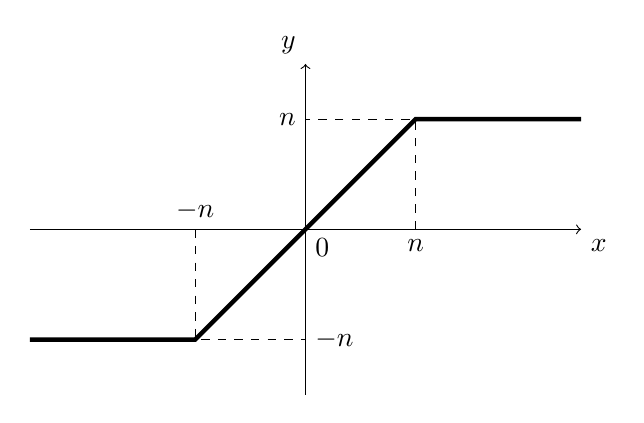
\begin{tikzpicture}
	[declare function={N = 2;}, scale=0.7]

	% axis
	\draw[thin,->] (-5,0) -- (5,0) node[anchor=north west] {$x$};
	\draw[thin,->] (0,-3) -- (0,3) node[anchor=south east] {$y$};

	% dashed
	\draw[dashed] ( N,0) node[below] { $n$} -- ( N, N) -- (0, N) node[left]   {$n$};
	\draw[dashed] (-N,0) node[above] {$-n$} -- (-N,-N) -- (0,-N) node[right] {$-n$};

	% function
	\draw[ultra thick] (-5,-N) -- (-N,-N) -- (N,N) -- (5,N);

	\coordinate[label=below right:$0$] (o) at (0,0);
	%\draw[step=1cm,gray,ultra thin] (-6,-N-1) grid (6,4);

	\end{tikzpicture}
	\caption{Approximation of the identity map.}
\end{figure}
%\fg[Approximation of the identity map.]{0.3}{identity_approximation}
s.t.:
\begin{equation*}
	\int_{G}f_n (X)\mathrm{d}\mathbb{P}=\int_{G}\mathbb{E}[f_n (X)]\mathrm{d}\mathbb{P}
\end{equation*}
Finally, applying the monotone convergence theorem as $n\to\infty$
\begin{equation*}
	\int_{G}X\mathrm{d}\mathbb{P}=\int_{G}\mathbb{E}[X]\mathrm{d}\mathbb{P}
\end{equation*}
\end{proof}
\item \textbf{Contractivity in $\mathcal{L}^p(\Omega,\mathcal{F},\mathbb{P})$}, $p\geq 1$ \\
\begin{equation*}
	X \in \mathcal{L}^p(\Omega,\mathcal{F},\mathbb{P})\implies \mathbb{E}[X|\mathcal{G}]\in \mathcal{L}^p(\Omega,\mathcal{G},\mathbb{P})
\end{equation*}
Indeed, is a consequence of the Jensen's inequality:
If $\Phi : \mathbb{R}\to\mathbb{R}$ is convex and $\mathbb{E}[|\Phi(X)|]<+\infty $, then:
\begin{equation*}
\Phi(\mathbb{E}[X])\leq\mathbb{E}[\Phi(X)]
\end{equation*}
(that also holds for conditional expectations $\Phi(\mathbb{E}[X|\mathcal{G}])\leq\mathbb{E}[\Phi(X)|\mathcal{G}]$). In our case $ \Phi(X)=|X|^p$.
\begin{teo}
	$X$ r.v. with $\mathbb{E}[|X|^p]<+\infty $\\
	$V$ $\mathcal{G}$-measurable random variable with $\mathbb{E}[|V|^q]<+\infty$ with $\frac{1}{p}+\frac{1}{q}=1$ conjugate index.
	Then
	\begin{equation*}
		\mathbb{E}[V\cdot X|\mathcal{G}]=V\cdot \mathbb{E}[X|\mathcal{G}]
	\end{equation*}
\end{teo}
\begin{proof}
	$V$ indicator function $V=\ind_G \quad G\in\mathcal{G}$ ($V$ $\mathcal{G}$-measurable), then, by definition of conditional expectation, $\forall G'\in \mathcal{G}$:
\begin{equation*}
	\begin{split}
		\int_{G'}\mathbb{E}[\ind_G \cdot X|\mathcal{G}]\mathrm{d}\mathbb{P}&=
		\int_{G'}\ind_G \cdot X\mathrm{d}\mathbb{P}=
		\int_{G'\cap G}X\mathrm{d}\mathbb{P}=\\
		&=\int_{G'\cap G}\mathbb{E}[X|\mathcal{G}]\mathrm{d}\mathbb{P}=
		\int_{G'}\ind_G \cdot\mathbb{E}[ X|\mathcal{G}]\mathrm{d}\mathbb{P}
	\end{split}
\end{equation*}
by the arbitrarity of $G'$: 
	\begin{equation*}
	\mathbb{E}[\ind_G\cdot X|\mathcal{G}]=\ind_G\cdot \mathbb{E}[X|\mathcal{G}]
\end{equation*}
by linearity:
\begin{equation*}
	\mathbb{E}[V\cdot X|\mathcal{G}]=V\cdot \mathbb{E}[X|\mathcal{G}] \qquad\forall V \text{simple and  $\mathcal{G}$-measurable}  
\end{equation*} 
If $V>0$, $V=\sup_{n\geq 1}V_n$ with $V_n$ simple   $\mathcal{G}$-measurable, so:
\begin{equation*}
	\mathbb{E}[V\cdot X|\mathcal{G}]=
	\sup_{n\geq 1}\mathbb{E}[V_n\cdot X|\mathcal{G}]=
	\sup_{n\geq 1}V_n\cdot \mathbb{E}[X|\mathcal{G}] =
	V\cdot \mathbb{E}[X|\mathcal{G}]
\end{equation*} 
If $V$ is real we can write $V=V^{+}-V^{-}$ and the thesis follows.
\end{proof}
\begin{teo}
If $X$ r.r.v. with $\mathbb{E}[|X|^2]<+\infty $, then:\\
$Z$ $\mathcal{G}$-measurable random variable with $\mathbb{E}[|Z|^2]<+\infty$\\
\begin{equation*}
	\mathbb{E}[|X-Z|^2]=\mathbb{E}[\ |X-\mathbb{E}[X|\mathcal{G}]|^2\ ]+\mathbb{E}[\ |\mathbb{E}[X|\mathcal{G}]-Z|^2\ ]
\end{equation*}
In particular:
\begin{equation*}
	\mathbb{E}[|X-Z|^2]=\min_{Z\in\mathcal{L}^2(\Omega,\mathcal{F},\mathbb{P})}\mathbb{E}[|X-\mathbb{E}[X|\mathcal{G}]|^2]
\end{equation*}
\end{teo}
\begin{proof}
	\begin{equation*}
		\begin{split}
			\mathbb{E}[|X-Z|^2]&=\mathbb{E}[\ [(X-\mathbb{E}[X|\mathcal{G}])+(\mathbb{E}[X|\mathcal{G}]-Z)]^2\ ]\\
			&=\mathbb{E}[\ |X-\mathbb{E}[X|\mathcal{G}]|^2\ ]+\mathbb{E}[\ |\mathbb{E}[X|\mathcal{G}]-Z|^2\ ]\\
			&\qquad+2\cdot\mathbb{E}[\ [(X-\mathbb{E}[X|\mathcal{G}])(\mathbb{E}[X|\mathcal{G}]-Z)]\ ]
		\end{split}		
	\end{equation*}
We only need to prove that the last term is zero.
By Projective property:
\begin{equation*}
\mathbb{E}[\ [(X-\mathbb{E}[X|\mathcal{G}])(\mathbb{E}[X|\mathcal{G}]-Z)]\ ]=
\mathbb{E}[\mathbb{E}[\ [(X-\mathbb{E}[X|\mathcal{G}])(\mathbb{E}[X|\mathcal{G}]-Z)]\ ]|\mathcal{G}]
\end{equation*}
$\mathbb{E}[X|\mathcal{G}]-Z$ is $\mathcal{G}$-measurable, so:
\begin{equation*}
	\mathbb{E}[\mathbb{E}[\ [(X-\mathbb{E}[X|\mathcal{G}])(\mathbb{E}[X|\mathcal{G}]-Z)]\ ]|\mathcal{G}]=
	\mathbb{E}[(\mathbb{E}[X|\mathcal{G}]-Z)\cdot\mathbb{E}[\ [(X-\mathbb{E}[X|\mathcal{G}])]\ ]|\mathcal{G}]
\end{equation*}
Finally:
\begin{equation*}
	\begin{split}
		\mathbb{E}[\ [(X-\mathbb{E}[X|\mathcal{G}])]\ |\mathcal{G}]&=\mathbb{E}[X|\mathcal{G}]-\mathbb{E}[\ [(\mathbb{E}[X|\mathcal{G}])]\ |\mathcal{G}]\\
		&=\mathbb{E}[X|\mathcal{G}]-\mathbb{E}[X|\mathcal{G}]=0
	\end{split}
\end{equation*}
\end{proof}
\end{enumerate}

\section{Martingales}
\subsection{Introduction}
$ (\Omega,\mathcal{F},\mathbb{P}) $ $T$ set of times either $\mathbb{N}$ or $[0,\infty)$.
\begin{defi}
	A \textbf{filtration} on the probability space $ (\Omega,\mathcal{F},\mathbb{P})$ is a sequence ${\mathcal{F}_{t}:t=0,1,2, \ldots}$ of sub-sigma algebras of $\mathcal{F}$, such that for all $t$, $\mathcal{F}_{t} \subseteq \mathcal{F}_{t+1}$.
\end{defi}
The filtration represent our knowledge at successive times. This increases with time (i.e. we don't forget things).
\begin{defi}
	$(M_t)_{t\in T}$ is a Martingale w.r.t. a filtration $(\mathcal{F}_t)_{t\in T}$ of sub-$\sigma$-algebras of $\mathcal{F}$ if:
	\begin{enumerate}
		\item \textbf{(adaptedness)} $M_t$ is $\mathcal{F}_t$-measurable $\forall t\in T$
		\item \textbf{(integrability)} $\mathbb{E}[|M_t|]<+\infty \qquad\forall t$
		\item \textbf{(martinagle property)} $\forall s<t \qquad \mathbb{E}[M_t|\mathcal{F}_s]=M_s$
	\end{enumerate}
\end{defi}
\begin{exi}
	$(X_n)_{n\geq0}$ symmetric RW on $\mathbb{Z}$ starting from $0$.\\
	$X_n=\sum_{k=1}^{n}Y_k \qquad Y_k$ iid with $\mathbb{P}\{Y_k=1\}=\frac{1}{2}=\mathbb{P}\{Y_k=-1\}$ \\
	$(X_n)_{n\geq0}$ is a martingale w.r.t. $\{\mathcal{F}_n\}_{n\geq0}$ with $\mathcal{F}_n=\sigma(X_1,...,X_n)$.
\end{exi}
\begin{proof}
	We check the definition.
	\begin{enumerate}
		\item $X_n$ is $\mathcal{F}_n$-measurable.
		\item $X_n$ is integrable $(|X_n|\leq n)$.
		\item If $m<n$,
		\begin{equation*}
			\mathbb{E}[X_n|\mathcal{F}_m]=\mathbb{E}\left[ \sum_{k=m+1}^{n}Y_k+\sum_{k=1}^{m}Y_k|\mathcal{F}_m \right]  
		\end{equation*}
		The first sum is independent of $\mathcal{F}_m$, the second one is $\mathcal{F}_n$-measurable, so:
		\begin{equation*}
			\mathbb{E}[X_n|\mathcal{F}_m]=\mathbb{E}\left[ \sum_{k=m+1}^{n}Y_k \right]  +\sum_{k=1}^{m}Y_k=\sum_{k=m+1}^{n}\mathbb{E}[Y_k]+X_m=X_m
		\end{equation*}
	Since $\mathbb{E}[Y_k]=0$.
	\end{enumerate}
\end{proof}
\begin{exi}[Another martingale]
	$M_n=X^2_n-n \qquad(M_n)_{n\geq 0}$
	\begin{enumerate}
		\item $M_n$ is $\mathcal{F}_n$-measurable.
		\item $|M_n|\leq|X^2_n-n|\leq n^2+n<+\infty\implies\mathbb{E}[|M_n|]<+\infty$.
		\item 
		\begin{equation*}
			\begin{split}
				\mathbb{E}[X_n|\mathcal{F}_m]&=\mathbb{E}[X^2_n-n|\mathcal{F}_m]\\
				&=\mathbb{E}[X^2_n|\mathcal{F}_m]-\mathbb{E}[n|\mathcal{F}_m]=\\
				&=\mathbb{E}\left[ \left( \sum_{k=1}^{m}Y_k+\sum_{k=m+1}^{n}Y_k \right)  ^2|\mathcal{F}_m \right]  -n=\\
				&=\mathbb{E}\left[ \left( \sum_{k=1}^{m}Y_k \right)  ^2|\mathcal{F}_m \right]  +2\cdot\mathbb{E}\left[ \left( \sum_{k=1}^{m}Y_k \right)  \cdot\left( \sum_{k=m+1}^{n}Y_k \right)  |\mathcal{F}_m \right]  \\
				& \qquad +\mathbb{E}\left[ \left( \sum_{k=m+1}^{n}Y_k \right)  ^2|\mathcal{F}_m \right]  -n=\\
				&=X^2_m+2\cdot X_m\cdot \mathbb{E}\left[ \sum_{k=m+1}^{n}Y_k|\mathcal{F}_m \right]  +\mathbb{E}\left[ \left( \sum_{k=m+1}^{n}Y_k \right)  ^2 \right]  -n=\\
				&=X^2_m+2\cdot X_m\cdot0+\sum_{k=m+1}^{n}\mathbb{E}[Y_k^2]-n=\\
				&=X^2_m+(n-m)-n=X^2_m-m=M_m
			\end{split}			
		\end{equation*}
	Since $\mathbb{E}[Y_k]=0$ and $\mathbb{E}[Y_k^2]=1$.
	\end{enumerate}
\end{exi}
\subsection{Stopping time}
$T$ stopping time of the filtration $(\mathcal{F}_t)_{t\in T}$ (i.e. $\{T\leq t\}\in\mathcal{F}_t \qquad\forall t\geq0$)\\
We call \textbf{stopped martingale at time} $T$: $M^{IT}=(M_{\min{(T,t)}})_{t\geq0}$.
\begin{teo}[Stopping Theorem]
	$(M_{\min{(T,t)}})_{t\geq0}$ is a martingale w.r.t. the same filtration $(\mathcal{F}_t)_{t\in T}$ and in particular:
	\begin{equation}
		\mathbb{E}[M_{\min{(T,t)}}]=\mathbb{E}[M_{0}]
	\end{equation}
\end{teo}
\begin{rem}
	A martingale $(M_t)_{t\in T}$ necesseraly has constant means by:
	\begin{equation*}
		\mathbb{E}[M_{T}]=\mathbb{E}[\mathbb{E}[M_{T}|\mathcal{F}_s]]=\mathbb{E}[M_{0}] \qquad \forall s<t
	\end{equation*} 
\end{rem}
\begin{exi}
	$(X_n)_{n\geq0}$ symmetric RW on $\mathbb{Z}$ starting from $0$ and $a,b\in\mathbb{N}$ or $a,b>0$.\\
	$X_n=\sum_{k=1}^{n}Y_k \qquad Y_k$ iid with $\mathbb{P}\{Y_k=1\}=\frac{1}{2}=\mathbb{P}\{Y_k=-1\}$ \\
	We want to compute the exit probability from $(-a,b)$ either from $-a$ or $b$ and the mean exit time $T=\min{(n\geq1|X_n=-a \text{ or } X_n=b)}$. \\
	Consider the martingales $(X_n)_{n\geq0}$ and $(X^2_n-n)_{n\geq0}$ and apply the stopping theorem: 
	\begin{equation*}
		\mathbb{E}[X^2_{T\land n}-T\land n]=\mathbb{E}[0]=0
	\end{equation*}
	\begin{equation}
		\mathbb{E}[X^2_{T\land n}]=\mathbb{E}[T\land n]
		\label{eq:applying-stopping-theorem-example}
	\end{equation}
Thus $ \mathbb{E}[T\land n]\leq\max{(a^2,b^2)} $ because $  |X^2_{T\land n}|\leq\max{(a^2,b^2)}$, thus we have: $\mathbb{E}[T]=\sup_{n\geq1}\mathbb{E}[T\land n]$\\
	Applying the stopping theorem to $(X_n)_{n\geq0}$:
	\begin{equation*}
		\mathbb{E}[X_{T\land n}]=\mathbb{E}[X_0]=0
	\end{equation*}
\begin{equation*}
	\mathbb{E}[X_{T\land n}]\leq\max{(a,b)}
\end{equation*}                                                 
Using dominated convergence:                                    
\begin{equation*}                                               
	\mathbb{E}[X_{T}]=\lim_{n\to\infty}\mathbb{E}[X_{T\land n}]=0
\end{equation*}
\begin{equation*}                                               
	0=-a\cdot\mathbb{P}\{X_T=-a\}+b\cdot\mathbb{P}\{X_T=b\}
\end{equation*}
Recalling that:
\begin{equation*}                                               
	\mathbb{P}\{X_T=-a\}+\mathbb{P}\{X_T=b\}=1
\end{equation*}
Solving the system:
\begin{equation*}                                               
	\mathbb{P}\{X_T=-a\}=\frac{b}{a+b} \qquad \mathbb{P}\{X_T=b\}=\frac{a}{a+b}
\end{equation*}
Then using monotone convergence on the RHS on \eqref{eq:applying-stopping-theorem-example} and dominated convergence on the LHS as $n\to\infty$ we obtain:
\begin{equation*}  
	\begin{split}
		\mathbb{E}[T]&=\mathbb{E}[X^2_T]=a^2\cdot\mathbb{P}\{X_T=-a\}+b^2\cdot\mathbb{P}\{X_T=b\}=\\&=\frac{a^2b}{a+b}+\frac{ab^2}{a+b}=ab
	\end{split}                                             
\end{equation*}
\end{exi}
\begin{rem}
	Note the resemblance of this result with the mean ending time starting from $i$ in the gambler's ruin problem:
	\begin{equation*}                                               
		\mathbb{E}_i[T]=i(N-i)
	\end{equation*}
\end{rem}
\begin{rem}[Warning]
	It is not always possible to take the limit $n\to\infty$ to find $ \mathbb{E}[M_{\min{(T,t)}}]=\mathbb{E}[M_{t}] $
\end{rem}
\begin{exi}
	$(X_n)_{n\geq0}$ symmetric RW on $\mathbb{Z}$ starting from $0$.\\
	$S=\min{\{n\geq1: X_n=1\}}$ \\
	Stopping theorem $\mathbb{E}[X_{\min{(S,n)}}]=0 $ but $\mathbb{E}[X_{S}]=1 $, therefore:
	\begin{equation*}
		\lim_{n\to\infty}\mathbb{E}[X_{\min{(S,n)}}]\neq\mathbb{E}[X_{S}]
	\end{equation*}
\end{exi}
\textbf{How to find martingales of a discrete time MC?}
\begin{teo}
	$(X_n)_{n\geq0}$ MC with values in a discrete set $I$\\
	$f:I\to\mathbb{R}\quad $ s.t. $ \mathbb{E}[|f(X_n)|]<+\infty$, then:
	\begin{equation}
		M_n=f(X_n)-\sum_{k=0}^{\textbf{n-1}}(Pf(X_k)-f(X_k))
	\end{equation}
$(M_n)_{n\geq0}$ is a martingale w.r.t. the natural filtration of $(X_n)_{n\geq0}$.
Where $(Pf)(j)=\sum_{j'\in I}p_{jj'}f(j')$.
\end{teo}
\begin{proof}
We check the definition:
	\begin{enumerate}
		\item $M_n$ is $\mathcal{F}_n$-measurable.
		\item $M_n$ is integrable.\\
		$\mathbb{E}[|f(X_n)|]<+\infty$ by assumption $\forall n$.\\
		$\mathbb{E}[|Pf(X_k)|]=\mathbb{E}[|\mathbb{E}[f(X_{k+1})|\mathcal{F}_k]|]<+\infty$
		The equality holds since:
		\begin{equation*}
			\mathbb{E}[f(X_{k+1})|\mathcal{F}_k]=Pf(X_k)
		\end{equation*}
	indeed for $m<n$:
	\begin{equation*}
		\mathbb{E}[f(X_{n})|\mathcal{F}_m]=P^{n-m}f(X_m)
	\end{equation*}
because:
		\begin{equation*}
			\begin{split}
				\mathbb{E}[f(X_{n})|\mathcal{F}_m]&=\mathbb{E}[\mathbb{E}[f(X_{n})|\mathcal{F}_{n-1}]|\mathcal{F}_m]\\&=\mathbb{E}[Pf(X_{n-1})|\mathcal{F}_m]\\&=\mathbb{E}[P^2f(X_{n-2})|\mathcal{F}_m]=...
			\end{split}		
	\end{equation*}
		\item For $n>m$:
		\begin{equation*}
			\begin{split}
			\mathbb{E}[M_{n}|\mathcal{F}_m]&=\mathbb{E}\left[ f(X_n)-\sum_{k=0}^{n-1}(Pf(X_k)-f(X_k))\bigg|\mathcal{F}_m \right]  \\
			&=\mathbb{E}\left[ f(X_n)-f(X_m)-\sum_{k=m}^{n-1}(Pf(X_k)-f(X_k))\bigg|\mathcal{F}_m \right]\\
			&\qquad +\underbrace{f(X_m)-\sum_{k=0}^{m-1}(Pf(X_k)-f(X_k))}_{M_m}\\
			&=(*)+M_m
			\end{split}		
		\end{equation*}
		The last term is $M_m$ so it suffices to show that the first term is zero. It is equal to:
		\begin{equation*}
			\begin{split}
				(*) &=\mathbb{E}\left[ \mathbb{E}\left[ f(X_n)-f(X_m)-\sum_{k=m}^{n-1}(Pf(X_k)-f(X_k))\bigg|\mathcal{F}_{n-1} \right]  \bigg|\mathcal{F}_m \right]  =\\
				&=\mathbb{E}\left[ \cancel{Pf(X_{n-1})}-f(X_m)-\cancel{Pf(X_{n-1})}+f(X_{n-1})-\sum_{k=m}^{n-2}(\ldots )\bigg|\mathcal{F}_m \right]  =\\
				&=\mathbb{E}\left[ f(X_{n-1})-f(X_m)-\sum_{k=m}^{n-2}(Pf(X_k)-f(X_k))\bigg|\mathcal{F}_m \right]  =\\
				&=\text{iterating...}=\mathbb{E}[f(X_m)-f(X_m)]=0
			\end{split}		
		\end{equation*}
	\end{enumerate}
\end{proof}
\begin{exi}
	$(X_n)_{n\geq0}$ symmetric RW on $\mathbb{Z}$ starting from $0$.\\
	$f(x)=x^2$.\\
	$\left(M_n=f(X_n)-\sum_{k=1}^{n-1}\left(Pf(X_k)-f(X_k)\right)\right)$
	\begin{equation*}
		Pf(i)=p_{i,i+1}f(i+1)+p_{i,i-1}f(i-1)=\frac{1}{2}(i+1)^2+\frac{1}{2}(i-1)^2=i^2+1
	\end{equation*}
\begin{equation*}
	Pf(i)-f(i)=1
\end{equation*}
\begin{equation*}
	\sum_{k=0}^{n-1}Pf(i)-f(i)=n \implies M_n=X_n^2-n
\end{equation*}
\end{exi}
\begin{rem}
	If you add a constant to a martingale it remains a martingale.
\end{rem}







% lecture 15/12

\begin{teo}
	[Martingale stopping theorem] Let $\mathbb{T}$ be a set of times, $( M_{t})_{t\in \mathbb{T}}$ a Martingale w.r.t. a filtration $(\mathcal{F}_{t})_{t\in \mathbb{T}}$ and $T$ a stopping time w.r.t. $(\mathcal{F}_{t})_{t\in \mathbb{T}}$. Then $( M_{T\land t})_{t\in \mathbb{T}}$ is still a Martingale w.r.t. the same filtration $(\mathcal{F}_{t})_{t\in \mathbb{T}}$. In particular:
	\begin{equation*}
		\mathbb{E}[ M_{T\land t}] =\mathbb{E}[ M_{0}]
	\end{equation*}
\end{teo}
\begin{proof}
	(case with $T$ \textit{discrete} stopping time\footnote{Otherwise boring approximation stuff...}) We have to check the three properties.
	\begin{enumerate}
		\item (adaptedness) i.e. $\forall t$, $M_{T\land t}$ is $\mathcal{F}_{t}$-measurable.
		      
		      \begin{equation*}
		      	T\ \text{discrete} \ \ \Rightarrow \ \ T=\sum\limits _{r\in D} r\ind_{\{T\leq r\}}
		      \end{equation*}
		      
		      $\{T=r\} \in \mathcal{F}_{r}$ because $T$ is a stopping time.\footnote{$\{T=r\} =\{T\leqslant r\} \setminus \bigcup _{n\geqslant 1}\left\{t\leqslant r-\frac{1}{n}\right\}$. We have to use inequalities.} We can decompose the RV, one up to time $t$ and one after $t$:
		      
		      \begin{equation*}
		      	M_{T\land t} =\sum _{r\in D\cap [ 0,t]}\underbrace{M_{r}\ind_{\{T=r\}}}_{ \begin{array}{l}
		      		\mathcal{F}_{r}\text{-measurable}\\
		      		r\leq t\\
		      		\Rightarrow \mathcal{F}_{t}\text{-measurable}
		      		\end{array}} +\underbrace{M_{t}}_{\mathcal{F}_{t}\text{-measurable}}\underbrace{\ind_{\{T >t\}}}_{\{T\leq t\}^{C} \in \mathcal{F}_{t}}
		      \end{equation*}
		      
		      as a result, $M_{T\land t}$ is $\mathcal{F}_{t}$-measurable.
		\item (integrability) i.e. $\mathbb{E}[| M_{T\land t}| ] < +\infty $. We can use again the decomposition. Moreover, since $D$ is discrete, this implies that $D\cap [ 0,t]$ is \textit{finite} for any $t$. Thus:
		      
		      \begin{equation*}
		      	| M_{T\land t}| \leq \sum _{r\in D\cap [ 0,t]}| M_{r}| \ind_{\{T=r\}} +| M_{t}| \ind_{\{T< t\}}
		      \end{equation*}
		      
		      is a finite sum of integrable RVs.
		\item $\mathbb{E}[ M_{T\land t} |\mathcal{F}_{s}] =M_{T\land s}$ for any $s< t$, i.e. we have to check that
		      
		      \begin{equation*}
		      	\forall A\in \mathcal{F}_{s} :\ \ \int _{A} M_{T\land s} d\mathbb{P} =\int _{A} M_{T\land t} d\mathbb{P}
		      \end{equation*}
		      
		      Notice that both $A\cap \{T\leq s\}$ and $A\cap \{T >s\}$ belong to $\mathcal{F}_{s}$.
		      
		      Computing:
		      
		      \begin{align*}
		      	\int _{A} M_{T\land s} d\mathbb{P} & =\int _{A\cap \{T\leq s\}} M_{T} d\mathbb{P} +\int _{A\cap \{T >s\}} M_{s} d\mathbb{P}                                                                     \\
		      	                                   & =\int _{A\cap \{T\leq s\}} M_{T} d\mathbb{P} +\int _{A\cap \{T >s\}} M_{\textcolor[rgb]{0.82,0.01,0.11}{t}} d\mathbb{P}                                    \\
		      	                                   & =\int _{A\cap \{T\leq s\}} M_{T} d\mathbb{P} +\underbrace{\int _{A\cap \{s< T\leq t\}} M_{t} d\mathbb{P}}_{( *)} +\int _{A\cap \{T >t\}} M_{t} d\mathbb{P} 
		      \end{align*}
		      
		      where in the second step we used the Martingale property of $( M_{t})_{t\in \mathbb{T}}$ and in the third we split the set. Notice that
		      
		      \begin{equation*}
		      	( *) =\int _{A\cap \{s< T\leq t\}} M_{t} d\mathbb{P} =\sum _{r\in D\cap ( s,t]}\int _{A\cap \{T=r\}} M_{t} d\mathbb{P}
		      \end{equation*}
		      
		      recall that $A\in \mathcal{F}_{s}$, $\{T=r\} \in \mathcal{F}_{r}$, $s< r$ then $A\cap \{T=r\} \in \mathcal{F}_{r}$ (the biggest). So using again the Martingale property for the given Martingale the integral in the sum can be written as
		      
		      \begin{equation*}
		      	\int _{A\cap \{T=r\}} M_{t} d\mathbb{P} =\int _{A\cap \{T=r\}} M_{r} d\mathbb{P}
		      \end{equation*}
		      
		      Summing up
		      
		      \begin{align*}
		      	\int _{A} M_{T\land s} d\mathbb{P} & =\int _{A\cap \{T\leq s\}} M_{T} d\mathbb{P} +\sum _{r\in D\cap ( s,t]}\int _{A\cap \{T=r\}} M_{r} d\mathbb{P} +\int _{A\cap \{T >t\}} M_{t} d\mathbb{P}                                                                                                                                          \\
		      	                                   & =\int _{A\cap \{T\leq s\}} M_{T} d\mathbb{P} +\sum _{r\in D\cap ( s,t]}\int _{A\cap \{T=r\}}\textcolor[rgb]{0.82,0.01,0.11}{M}\textcolor[rgb]{0.82,0.01,0.11}{_{T}} d\mathbb{P} +\int _{A\cap \{T >t\}}\textcolor[rgb]{0.82,0.01,0.11}{M}\textcolor[rgb]{0.82,0.01,0.11}{_{T\land t}} d\mathbb{P} \\
		      	?????                              & =\int _{A\cap \{T\leq s\}} M_{T\land t} d\mathbb{P} +\int _{A\cap \{s< T\leq t\}} M_{T\land t} d\mathbb{P} +\int _{A\cap \{T >t\}} M_{T\land t} d\mathbb{P}                                                                                                                                       \\
		      	                                   & =\int _{A} M_{T\land t} d\mathbb{P}                                                                                                                                                                                                                                                               
		      \end{align*}
	\end{enumerate}
\end{proof}



\textbf{Martingales of a continuous time Markov Chain}
\begin{teo}
	$( X_{t})_{t\geq 0}$ continuous time MC (regular..., FKE/BKE have a unique solution...). Consider $f:I\rightarrow \mathbb{R}$ such that $\mathbb{E}[| f( X_{t})| < +\infty $, $Q$ transition rate matrix, and $\mathbb{E}[| Qf( X_{s})| ] < +\infty \ \forall s$, then defining
		\begin{equation}
			M_{t} :=f( X_{t}) -\int _{0}^{t}( Qf)( X_{s}) ds
			\label{eq:martingale-ct}
		\end{equation}
	$( M_{t})_{t\geq 0}$ is a Martingale w.r.t. the natural filtration of the given MC $( X_{t})_{t\geq 0}$, namely the collection $(\mathcal{F}_{t})_{t\geq 0}$ of $\mathcal{F}_{t} :=\sigma ( X_{s} |s\leq t)$.
\end{teo}
\begin{rem}
	Compare \eqref{eq:martingale-ct} with the discrete-time analog:
	\begin{equation*}
		f( X_{n}) -\sum _{k=0}^{n-1}( Pf( X_{k}) -f( X_{k}))
	\end{equation*}
\end{rem}
\begin{proof}
	Recall that $\mathbb{E}[ f( X_{t}) |\mathcal{F}_{s}] =( P_{t-s} f)( X_{s})$ where $P_{t-s} =( p_{ij}( t-s))_{i,j\in I}$. We check the Martingale property:
	\begin{equation*}
		\mathbb{E}[ M_{t} |\mathcal{F}_{s}] \questeq M_{s}
	\end{equation*}
	We begin the computation
	\begin{align*}
		\mathbb{E}[ M_{t} |\mathcal{F}_{s}] =\mathbb{E}\left[ f( X_{t}) -\int _{0}^{t} Qf( X_{r}) dr|\mathcal{F}_{s}\right] & \questeq f( X_{s}) -\int _{0}^{s} Qf( X_{r}) dr=M_{s} 
	\end{align*}
	$\int _{0}^{t} =\int _{0}^{s} +\int _{s}^{t}$ \ \ \ ?????
	\begin{align*}
		\mathbb{E}\left[ f( X_{t}) -f( X_{s}) -\int _{s}^{t} Qf( X_{r}) dr|\mathcal{F}_{s}\right] & \questeq 0                                                                        \\
		\mathbb{E}[ f( X_{t}) -f( X_{s}) |\mathcal{F}_{s}]                                        & \questeq\mathbb{E}\left[\int _{s}^{t} Qf( X_{r}) dr|\mathcal{F}_{s}\right] =( *) 
	\end{align*}
	then since the conditional expectation is essentially an integral, by Fubini's theorem and remembering that $( P_{r-s} Qf)( j) =\sum _{jk} p_{ij}( r-s) q_{jk} f( k)$, we have the FKE, $\dotsc =\frac{d}{dr}\sum _{k} p_{ik}( r-s) f( k)$
	\begin{align*}
		( *) & =\int _{s}^{t}\mathbb{E}[ Qf( X_{r}) |\mathcal{F}_{s}] dr \\
		     & =\int _{s}^{t}( P_{r-s} Qf)( X_{s}) dr                    \\
		     & =\int _{s}^{t}\frac{d}{dr}( P_{r-s} f)( X_{s}) dr         \\
		     & =( P_{r-s} f)( X_{s}) |_{s}^{t}                           \\
		     & =P_{t-s} f( X_{s}) -f( X_{s})                             \\
		     & =\mathbb{E}[ f( X_{t}) |\mathcal{F}_{s}] -f( X_{s})       \\
		     & =\mathbb{E}[ f( X_{t}) -f( X_{s}) |\mathcal{F}_{s}]
	\end{align*}
\end{proof}
\textbf{Application/example.}

Computation of the mean depletion time of an $M/M/1$ queue (i.e. mean extinction time of a population).

		$( X_{t})_{t\geq 0}$ where $X_{t}$ is the number of individuals in the system, with $1$ counter. Suppose the system can host at most $N$ individuals\footnote{to avoid technical problems of integrability.} (it's not exactly a $M/M/1$ queue). The set of states is then $\{0,1,\dotsc ,N\}$.
\begin{equation*}
	Q=\begin{bmatrix}
	-\lambda  & \lambda  & 0 & 0 & \cdots  & 0\\
	\mu  & -( \lambda +\mu ) & \lambda  & 0 & \cdots  & 0\\
	\vdots  & \ddots  & \ddots  & \ddots  & \ddots  & \vdots \\
	0 & \cdots  & 0 & \mu  & -( \lambda +\mu ) & \lambda \\
	0 & \cdots  & 0 & 0 & \mu  & -\mu 
	\end{bmatrix} ,\ \ \lambda < \mu 
\end{equation*}
We consider as initial state $n$, where $n\ll N$, and define
\begin{equation*}
	T=\min\{t\geq 0|X_{t} =0\} ,
\end{equation*}
we want to compute $\mathbb{E}_{n}[ T]$ using the Martingales theorem.

Consider $f( n) =n$:
\begin{align*}
	\text{if} \ n >0,\ \ Qf( n) & =\mu f( n-1) -( \lambda +\mu ) f( n) +\lambda f( n+1) \\
	                            & =\mu ( n-1) +( \lambda +\mu ) n+\lambda ( n+1)        \\
	                            & =\lambda -\mu                                         \\
	\text{if} \ n=0,\ \ Qf( 0)  & =\lambda ( f( 1) -f( 0)) =\lambda                     
\end{align*}
The martingale is
\begin{equation*}
	X_{t} -\int _{0}^{t}( \lambda \ind_{\{X_{s} =0\}} +( \lambda -\mu )\ind_{\{X_{s}  >0\}}) ds
\end{equation*}
Martingale stopping theorem:
\begin{equation*}
	\mathbb{E}_{n}\left[ X_{T\land t} -\int _{0}^{T\land t}\left(\cancel{\lambda \ind_{\{X_{s} =0\}}} +( \lambda -\mu )\ind_{\{X_{s}  >0\}}\right) ds\right] =n
\end{equation*}
when $s< T$ you have not yet reached $0$, so the first $\ind$ is zero and the second is one.
\begin{equation}
	\mathbb{E}_{n}[\underbrace{X_{T\land t}}_{\geq 0} +( \mu -\lambda )( T\land t)] =n
	\label{eq:example-ct-mart}
\end{equation}
thus
\begin{equation*}
	\mathbb{( \mu -\lambda ) E}_{n}[ T\land t] \leq n\ \ \Rightarrow \ \ \text{when} \ t\rightarrow \infty :\ \mathbb{E}_{n}[ T] \leq \frac{n}{\mu -\lambda }
\end{equation*}
so $T$ is integrable. Back to \eqref{eq:example-ct-mart}
\begin{equation*}
	X_{T\land t}\xrightarrow[\text{a.s.}]{t\rightarrow \infty } X_{T} =0\ \ \Rightarrow \ \ ( \mu -\lambda )\mathbb{E}_{n}[ T] =n\ \ \Rightarrow \ \ \mathbb{E}_{n}[ T] =\frac{n}{\mu -\lambda }
		\end{equation*}

% Lecture 22/12/2021
\begin{teo}
	[Martingale Convergence Theorem] Given $( M_{t})_{t\geq 0}$ (with either $t\in \mathbb{N}$ or $t\in \mathbb{R}^{+}$) Martingale w.r.t. some filtration $(\mathcal{F}_{t})_{t\geq 0}$. If
	\begin{equation*}
		\sup _{t\geq 0}\mathbb{E}[| M_{t}| ] < +\infty 
	\end{equation*}
	then
	\begin{equation*}
		\lim\limits _{t\rightarrow +\infty } M_{t}
	\end{equation*}
	exists almost surely (may not be in $L^{1}$).
\end{teo}
\begin{exi}
	Consider $( X_{n})_{n\geq 0}$ symmetric RW on $\mathbb{Z}$.
	\begin{equation*}
		X_{0} =0\ \ \ \ X_{n} =\sum\limits _{k=1}^{n} Y_{k} \ \ \ \ Y_{k} \ \text{i.i.d.} \ \mathbb{P}( Y_{k} =\pm 1) =\frac{1}{2}
	\end{equation*}
	Let
	\begin{equation*}
		M_{n} =e^{\vartheta X_{n} -cn} ,\ \ c,\vartheta \in \mathbb{R}
	\end{equation*}
	\begin{enumerate}
		\item Find $c$ such that $( M_{n})_{n\geq 0}$ is a Martingale.
		\item Show that for such $c$ and all $\vartheta $, $M_{n}$ converges a.s., but not in $L^{1}$.
	\end{enumerate}



	For $( M_{n})_{n\geq 0}$ to be a Martingale, beside checking the two basic properties, we have to check that if $\mathbb{E}[ M_{n+1} |\mathcal{F}_{n}] \questeq M_{n}$. The first quantity is equal to:
	\begin{align*}
		\mathbb{E}[ M_{n+1} |\mathcal{F}_{n}] & =\mathbb{E}\left[ e^{\vartheta X_{n+1} -c( n+1)} |\mathcal{F}_{n}\right]                     \\
		                                      & =\mathbb{E}\left[ e^{\vartheta Y_{n+1} -c} e^{\vartheta X_{n} -cn} |\mathcal{F}_{n}\right]   \\
		                                      & =\mathbb{E}\left[ e^{\vartheta Y_{n+1}} |\mathcal{F}_{n}\right] e^{\vartheta X_{n} -c( n+1)} 
	\end{align*}
	thus
	\begin{align*}
		\mathbb{E}\left[ e^{\vartheta Y_{n+1}} |\mathcal{F}_{n}\right] e^{\vartheta X_{n} -c( n+1)} & \questeq e^{\vartheta X_{n} -cn}                                                                                                  \\
		\mathbb{E}\left[ e^{\vartheta Y_{n+1}}\right] e^{-c}                                        & \questeq 1                                                                                                                        \\
		e^{c}                                                                                       & \questeq \mathbb{E}\left[ e^{\vartheta Y_{n+1}}\right] =\frac{1}{2}\left( e^{\vartheta } +e^{-\vartheta }\right) =\cosh \vartheta 
	\end{align*}
	so
	\begin{equation*}
		c=\log\cosh \vartheta \ \ ( =c( \vartheta ))
	\end{equation*}
	With such $c$, $( M_{n})_{n\geq 0}$ is a Martingale
	\begin{equation*}
		| M_{n}| =M_{n} \ \ \Rightarrow \ \ \mathbb{E}[| M_{n}| ] =\mathbb{E}[ M_{n}] =\mathbb{E}[ M_{0}] =1
	\end{equation*}
	By Martingale convergence theorem, $M_{n}\xrightarrow[n\rightarrow \infty ]{\text{a.s.}} k$ and by the Law of Large Numbers we can compute $k$.
	\begin{equation*}
		X_{n} =\sum\limits _{k=1}^{n} Y_{k} \ \ \Rightarrow \ \ \frac{1}{n}\sum\limits _{k=1}^{n} Y_{k}\xrightarrow[n\rightarrow \infty ]{\text{a.s.}}\mathbb{E}[ Y_{1}] =0
	\end{equation*}
	then
	\begin{equation*}
		e^{\vartheta X_{n} -c( \vartheta ) n} =\Bigg( e^{\overbrace{\vartheta \frac{1}{n}\sum _{k=1}^{n} Y_{k}}^{\rightarrow 0} -c( \vartheta )}\Bigg)^{n} \sim \left( e^{-c( \vartheta )}\right)^{n}\rightarrow 0=k
	\end{equation*}
	since $c( \vartheta )  >0$, $e^{-c( \vartheta )} < 1$.

	Summing up:
	\begin{equation*}
		M_{n}\xrightarrow[n\rightarrow \infty ]{\text{a.s.}} 0\ \ \ \ \text{but} \ \ \ \ \mathbb{E}[ M_{n}] =1\ \ \Rightarrow \ \ M_{n} \nrightarrow 0\ \text{in} \ L^{1}
	\end{equation*}
\end{exi}
\subsection{Supermartingales and Submartingales}

Consider $( X_{t})_{t\geq 0}$ with either $t\in \mathbb{N}$ or $t\in \mathbb{R}^{+}$ and a filtration $(\mathcal{F}_{t})_{t\geq 0}$. We say that $( X_{t})_{t\geq 0}$ is a supermartingale (resp. submartingale) if
\begin{itemize}
	\item (adaptedness) $X_{t}$ is $\mathcal{F}_{t}$-measurable for all $t$.
	\item (integrability) $\mathbb{E}[| X_{t}| ] < +\infty $
	\item $\forall s< t$,\begin{align*}
	      \mathbb{E}[ X_{t} |\mathcal{F}_{s}] \leq X_{s} & ,\ \text{for supermartingales}\\
	      \mathbb{E}[ X_{t} |\mathcal{F}_{s}] \geq X_{s} & ,\ \text{for submartingales}
	\end{align*}
\end{itemize}
\begin{rem}
	A process is a Martingale if and only if it's both a sub- and super- Martingale.
\end{rem}
\begin{teo}
	If $( M_{t})_{t\geq 0}$ is a Martingale and $\varphi :\mathbb{R}\rightarrow \mathbb{R}$ is a \textbf{convex} (resp. \textbf{concave}) function such that $\mathbb{E}[| \varphi ( M_{t})| ] < +\infty $ for any $t$, then
	\begin{equation*}
		( \varphi ( M_{t}))_{t\geq 0}
	\end{equation*}
	is a \textbf{submartingale} (resp. \textbf{supermartingale}) w.r.t. the same filtration of $( M_{t})_{t\geq 0}$.
\end{teo}
\begin{proof}
	Consider $\varphi $ convex, using the Jensen inequality
	\begin{equation*}
		s< t\ \ \ \ \varphi ( M_{s}) =\varphi (\mathbb{E}[ M_{t} |\mathcal{F}_{s}]) \leq \mathbb{E}[ \varphi ( M_{t}) |\mathcal{F}_{s}]
	\end{equation*}
\end{proof}
\textbf{Examples.}

$\varphi ( x) =| x| $, $\varphi ( x) =| x| ^{2}$, $\varphi ( x) =\max\{0,x\}$.
\subsection{Doob-Meyer decomposition.}

Consider a submartingale $( X_{n})_{n\geq 0}$ with $n\in \mathbb{N}$ w.r.t. a filtration $(\mathcal{F}_{n})_{n\geq 0}$ then it can be written as
\begin{equation*}
	X_{n} =M_{n} +A_{n}
\end{equation*}
where $( M_{n})_{n\geq 0}$ is a martingale and $A_{n}$ is $\mathcal{F}_{n-1}$-measurable and increasing $A_{n+1} \geq A_{n}$ a.s.\footnote{$A_{n}$ is a \textit{predictable} process.}

\end{document}